\documentclass[12pt, landscape]{article}
\usepackage[a2paper]{geometry}
\usepackage[numbers]{natbib}
\usepackage{multicol}
\usepackage{blindtext}
\usepackage{setspace}
\usepackage{graphicx}
\usepackage{tikz}
\usepackage{float}
\usepackage{listings}
\usepackage{fancyvrb}
\usepackage{lipsum} % just for the example
\graphicspath{ {./images/} }
\setlength{\columnsep}{1cm}

%\doublespacing
%\documentclass[12pt,landscape]{article}
%\usepackage[a3paper]{geometry}

\title{Road Sign Recognition with CNN and RCNN}
\author{Aksel Tahir 6548051}
\date{11.05.2021}

\begin{document}
\maketitle
\tableofcontents
\pagebreak

\begin{multicols}{3}
\section{Introduction}
Road signs are a present system in virtually all road infrastructure. They are
of critical importance to interpreting correct road usage, road regulations and
route recommendations. Their presence is integral to the safe and functional
road use.

Contemporary road signs follow strict design rules to optimise their clarity of
intention. These rules allow them to be as easy as possible for human
interpretation. However, humans are prone to distraction, misinterpretation and
other general mistakes, which is why road sign recognition (RSR) algorithms are
a fast-advancing point of development in autonomous driving research.

Standard computer vision methods are not versatile enough to deal with the
plethora of different physical road conditions. This is why applying a deep
learning approach to the problem is necessary - A well crafted AI can exceed
even human vision in RSR.

In this project we propose an RSR solution using several different neural
network models and evaluating their performance. Since standard computer vision
methods are not versatile enough to deal with the plethora of different physical
road conditions, it is necessary to apply a deep learning approach to the
problem - A well crafted AI can exceed even human vision in RSR.

\section{Related Work}
With the advent of AI computing autonomous and assisted driving has been an area
of extensive research. Road sign recognition (RSR) systems are integral to the
field. The functional implementation of RSR systems depends on two related
issues - Road sign detection (RSD) and road sign classification (RSC). RSD
pertains to localising the relevant information from the data, and RSC to
identifying the data with its correct labels. There have already been a number
of outstanding studies in the detection and classification in
\citep{Classification1}, \citep{Classification2}, \citep{Classification3},
\citep{Classification4}, \citep{Classification5}.

In many RSR systems, the RSD part is done via conventional machine learning
methods. This approach is used by authors like Amal Bouti et al in
\citep{Recognition1}. The advantages of deep learning methods have made
themselves clear by now, but the author has chosen to discuss if SVMs do not still
have a place in RSR. In their findings, "the representation of the HOG features
and SVM greatly improves the results obtained and shows good results in terms of
accuracy. The linear SVM not only achieves high accuracy but also costs least
compared with another kernel function" \citep[6722 A. Bouti et al]{Recognition1}

[Add info about R-CNN too. That'd be pretty useful]

\section{Architectures}
This project is based entirely on image recognition, the models we have decided
to implement are all CNN-based. This section will describe them all in detail.

\subsection{CNN}
Recent decades have seen many advancements in representational learning from raw
data, with one of the most pertinent approaches to the method being the
varieties of CNN modelling. CNN dominates systems related to object recognition
and detection. This ubiquity in the field is one of the reasons that made us
choose it for our implementation.

Another major advantage of CNNs that led to our choice is the relatively sparse
pre-processing required to make a functioning model, compared to more
traditional image classifiers. The independent kernel optimisation that CNNs
learn, without much prior knowledge is hugely beneficial to implementation
complexity.

We have decided to implement two different CNN classifiers parallel to
each other, with the intention of seeing if our approaches and results will have
any significant differences. Aksel's CNN implementation will be referred to as
(CNN-A) and Kieran's as (CNN-K).

\subsection{R-CNN}
At the time of writing the R-CNN model has not been implemented.

\subsection{Faster R-CNN}
At the time of writing the Faster-R-CNN model has not been implemented.

\section{Dataset}
This project intends to use two datasets to conduct its study to ensure
flexibility and better insight. The data needed for detection differs from that
needed for classification, and many datasets do not meet both requirements. This
section will discuss our choices and their features.
\subsection{GTSRB - German Traffic Sign Recognition Benchmark}
The German Traffic Sign Recognition Benchmark is our first choice. It contains
43 data classes of road signs in Germany with each having enough examples to be
used in training.

\begin{itemize}
    \item As seen from the examples in Figure~\ref{fig:ex} dataset is only
    useful for classification purposes and not detection, since its items only
    feature photos of isolated road signs with no irrelevant data in the image.
    \begin{figure}[H]
        \centering
        \begin{tabular}{cc}
        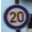
\includegraphics[scale=1.3]{ex1.png}&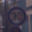
\includegraphics[scale=1.3]{ex2.png}\\
        
\includegraphics[scale=1.3]{ex3.png}&
\includegraphics[scale=1.3]{ex4.png}\\
        \end{tabular}
        \caption{Some examples of raw data from the dataset}
        \label{fig:ex}
    \end{figure}

    \item The dataset also contains unequal numbers of items in each class, as
    seen in Figure~\ref{fig:figure}, which introduces a challenge solved in
    Preprocessing.
    \begin{figure}[H]
        \centerline{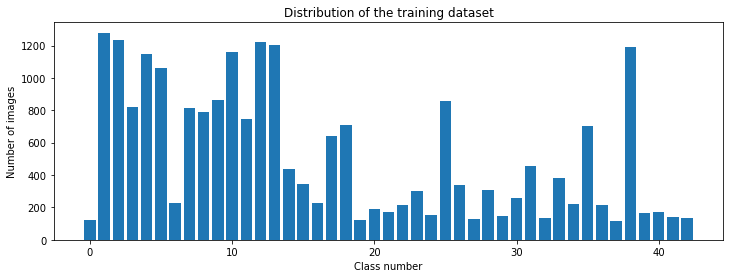
\includegraphics[scale = 0.5]{download.png}}
        \caption{Number of items in each class of GTSRB}
        \label{fig:figure}
    \end{figure}

  \end{itemize}

\subsubsection{Loading the dataset}
The ~50K images loaded from the dataset were split into two groups for training
and testing. The split was arbitrarily chosen to be 0.8/0.2 respectively. Out of
the 80\% chosen for training, 20\% were chosen for validation.

\color{red}
\begin{Verbatim}[fontsize=\small]
1   testRatio = 0.2 
2   # set aside 20% of images for testing, 80% for training
3   validationRatio = 0.2 
4   # of all training images, set aside 20% for validation
5
6   X_train, X_test, y_train, y_test = 
7   train_test_split(images, classNo, test_size=testRatio)
8   X_train, X_validation, y_train, y_validation = 
9   train_test_split(X_train, y_train, test_size=validationRatio)
10 
11  # X_train = ARRAY OF IMAGES TO TRAIN
12  # y_train = CORRESPONDING CLASS ID
\end{Verbatim}
\color{black}

\subsubsection{Preprocessing data}
There are quite a few tasks to be done with preprocessing the data from this
dataset. 
\begin{enumerate}
    \item
    The uneven distribution from Figure~\ref{fig:figure} needs to be processed
    to make every class equal. At the time of writing this has not been
    implemented.
    \item In CNN-A, the images are augmented - They are converted to a
    monochromatic greyscale and then undergo histogram equalisation. Finally
    their values are normalised from 0-255 to 0-1.
\end{enumerate}

\section{Implementation}

\subsection{CNN-A}
Modelling this CNN is very straightforward with Keras. The model we've chosen the
CNN-A implementation closely resembles LeNet (Figure~\ref{fig:figurelenet}),
proposed by Yann LeCun et al in 1998. The dataset we've trained the model upon
is the GTSRB.
\begin{figure}[H]
    \centerline{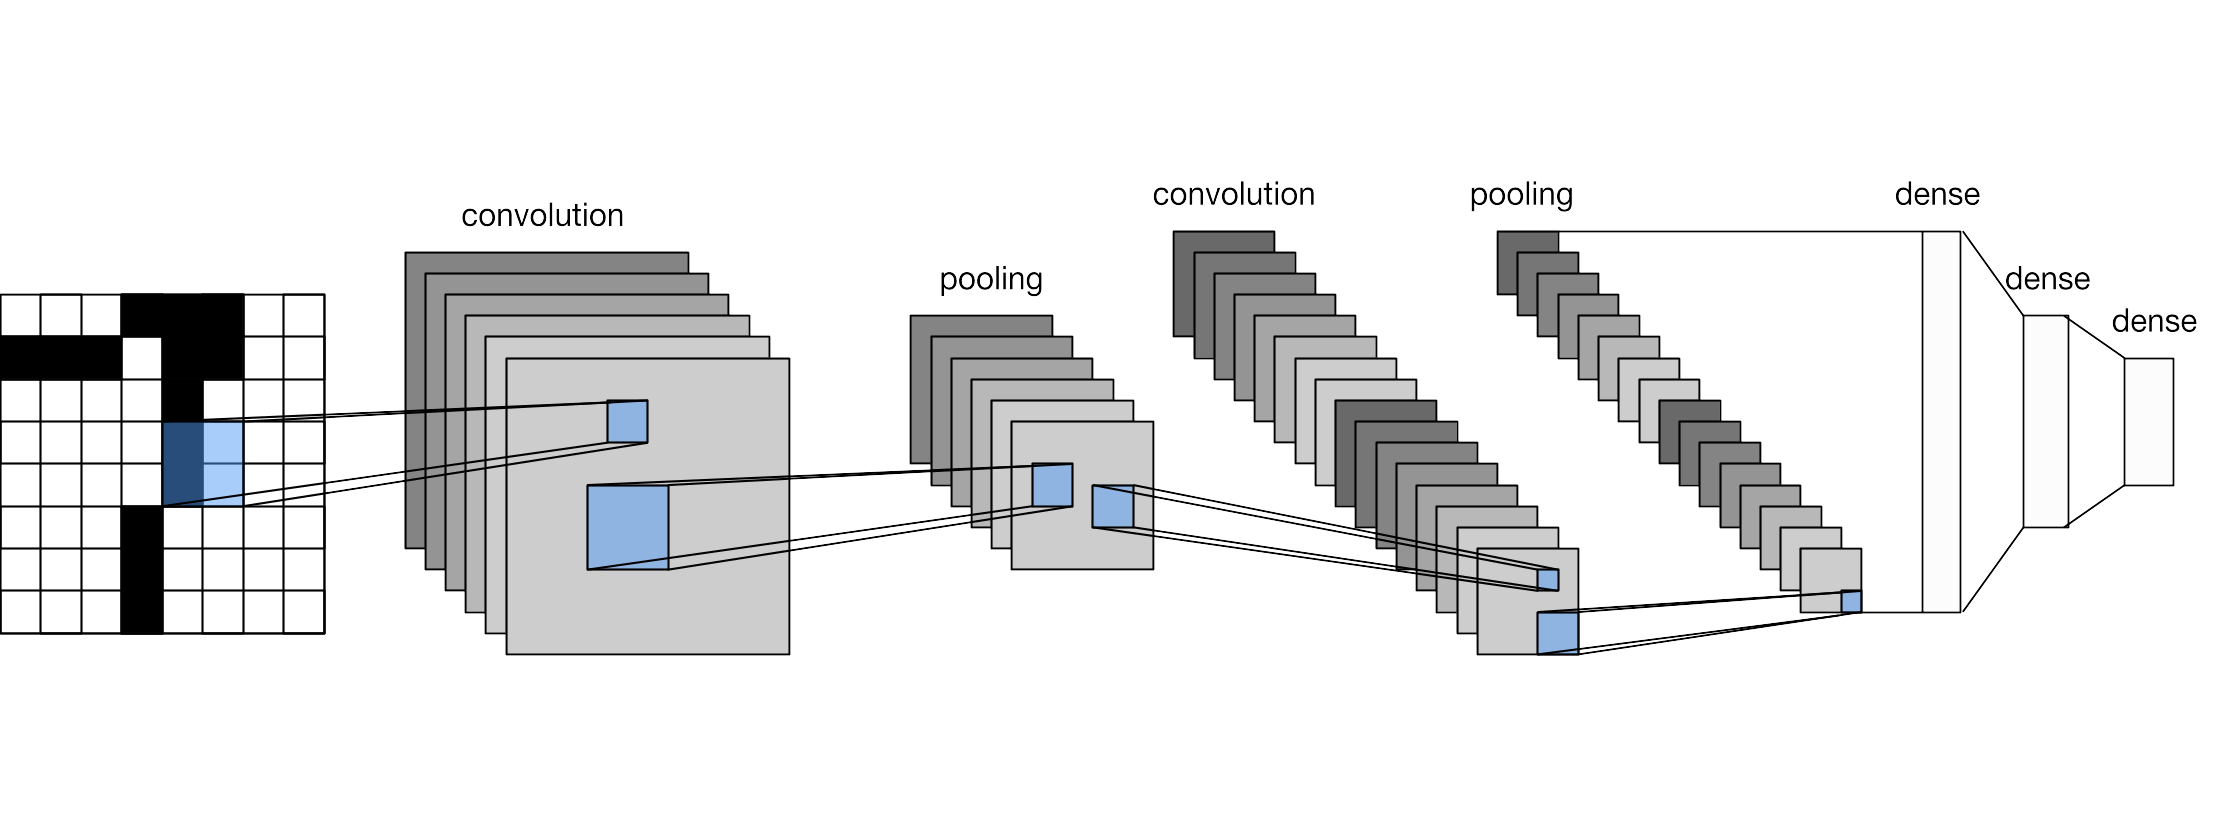
\includegraphics[scale = 0.2]{lenet.png}}
    \caption{Generic LeNet structure}
    \label{fig:figurelenet}
\end{figure}

\subsubsection{Structure}
\begin{figure}[H]
    \centerline{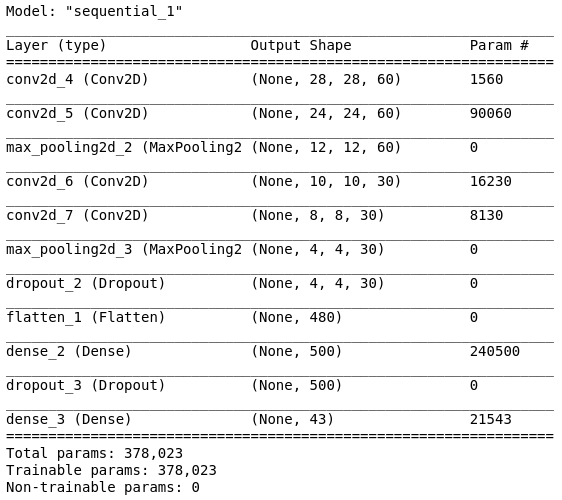
\includegraphics[scale = 0.5]{model.png}}
    \caption{Structure of our CNN-A model}
    \label{fig:figuremodel}
\end{figure}

The first two layers are convolutions. Layer 1 has a depth of 60, a filter size
of (5, 5), with relu activation. The second layer does the same. Following the
second convolution layer is a max polling layer. Following the LeNet model, we
use a (2,2) kernel size. It effectively downsizes the data by only selecting the
max value pixel for adjacent pixels.

Next we implement two other convolution layers with new parameters. Half the
number of filters and a filter size of (3,3). Their activation is also relu.
They're followed by a max pooling layer and a dropout layer to prevent
overfitting the model. 

Afterwards, the data is flattened and a dense layer with relu activation is
used. A second dropout layer prepares the model for the a last fully connected
dense layer with class number as size (ie. 43). Softmax is used to return the
probabilities of each class, and the model is compiled with the Adam optimiser.

\subsubsection{Performance}
\begin{figure}[H]
    \centering
    \begin{tabular}{cc}
    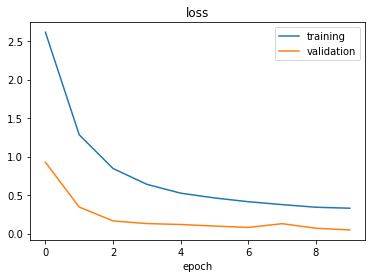
\includegraphics[scale=0.45]{accuracy1.png}&
    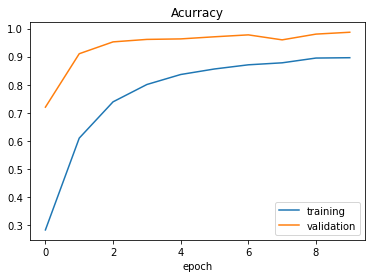
\includegraphics[scale=0.45]{accuracy2.png}\\
    \end{tabular}
    \caption{The Loss and Accuracy values throughout the epochs}
    \label{fig:acc}
\end{figure}
Within 10 epochs, the accuracy of both training and validation is above 0.98,
after which the model shows minimal improvements and the cost/ gain balance
becomes unreasonable.

This model achieved formidable results with relatively light training. After
roughly 30 minutes on Heron labs computers and 10 epochs the test accuracy
averaged in the 98th percentile. Figure~\ref{fig:acc} shows the relevant values
throughout training

\subsection{CNN-K}
Along with the difference in preprocessing, this implementation uses a different
model structure than the one in CNN-A. CNN-K studies two models, but in this
poster we will only look at the one reaching better results for the sake of
being concise.

\subsubsection{Structure}
\begin{figure}[H]
    \centerline{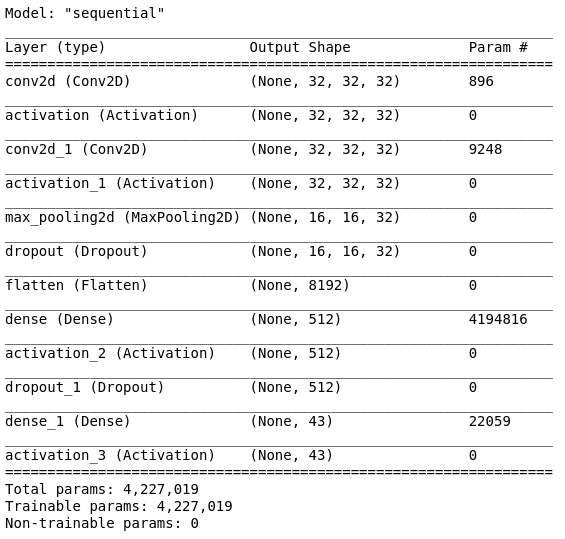
\includegraphics[scale = 0.5]{figuremodel1.png}}
    \caption{Structure of our CNN-K model}
    \label{fig:figuremodel1}
\end{figure}
Unlike the CNN-A implementation, this one beings with a convolutional layer of a
32,32,32 shape. An activation layer preceeds the second convolution. There is a
second activation, after which the data is reshaped in a max pooling grid.

It undergoes dropout and flattening, and the 8th layer is the first dense layer.
Another activation and dropout later, the data passes through the final dense
and activation layers and the output shape is 43, denoting the classes.

\subsubsection{Performance}
\begin{figure}[H]
    \centering
    \begin{tabular}{cc}
    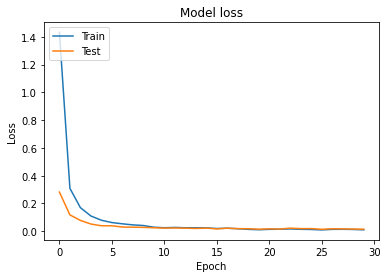
\includegraphics[scale=0.45]{Kresult1.png}&
    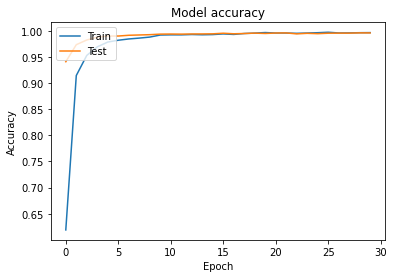
\includegraphics[scale=0.45]{Kresult.png}\\
    \end{tabular}
    \caption{The Loss and Accuracy values throughout the epochs}
    \label{fig1:acc}
\end{figure}
The model is fitted with 30 epochs, but as with the previous implementation, the
accuracy of both training and validation is above 0.98, after which the model
shows minimal improvements and the cost/gain balance becomes unreasonable.

\subsection{R-CNN}
\subsection{Faster R-CNN}

\section{Cross-Model Analysis}
\section{Conclusions}
data goes in and numbers come out and we don't question any of it


\bibliographystyle{unsrt}
\bibliography{References}
\nocite{*}
\end{multicols}
\end{document}